\documentclass{article}
\usepackage{amsmath}
\usepackage{amssymb}
\usepackage{graphicx}
\usepackage{hyperref}
\usepackage[version=4]{mhchem}


\begin{document}
(1984 China Middle School Math Contest) As shown in the figure, \(A B=B C=C A=A D . A H \perp C D\) at \(H, C P \perp B C\) at \(C\) and meets \(A H\) at \(P\). Prove that \(S=\frac{\sqrt{3}}{4} A P \times B D\), where \(S\) is the area of \(\triangle A B C\).\\
\centering
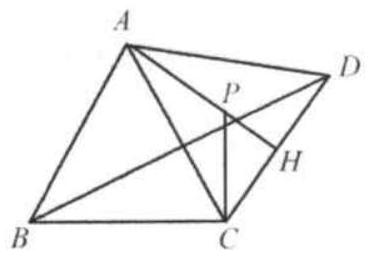
\includegraphics[width=\textwidth]{images/197(1).jpg}

Solution:
Method 1:\\
\(\operatorname{Draw} A E \perp B C\) at \(E\). \(E\) is the midpoint of \(B C\). \(H\) is the midpoint of \(D C\).\\
Connect EH. \(E H / / B D\).\\
Then \(\angle H E C=\angle D B C\).\\
Since \(A H \perp C D, A E \perp B C\), points \(A, H, C\), and \(E\) are concyclic. Therefore,\\
\centering
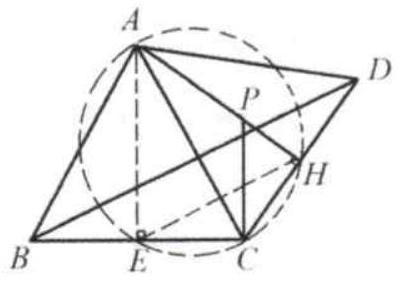
\includegraphics[width=\textwidth]{images/197(2).jpg}\\
\(\angle H A C=\angle H E C=\angle D B C\).


We know that \(\angle E A C=\angle E H C=\angle B D C=30^{\circ}\).\\
\(\angle P C A=90^{\circ}-60^{\circ}=30^{\circ}\). So \(\angle P C A=\angle B D C\).\\
Thus \(\triangle A C P \sim \triangle B D C\).\\
So \(\frac{A P}{B C}=\frac{A C}{B D} \Rightarrow A P \times B D=B C \times A C \Rightarrow\) \(S_{A B C}=\frac{\sqrt{3}}{4} A C^{2}=\frac{\sqrt{3}}{4} B C \times A C=\frac{\sqrt{3}}{4} A P \times B D\).

Method 2:\\
Let the point of intersection of \(B D\) and \(A H\) be \(Q\).\\
Since \(A H \perp C D, A C=A D, \angle A C Q=\angle A D Q\).\\
Since \(A B=A D, \angle A D Q=\angle A B Q\).\\
\(\angle A B Q=\angle A C Q\).\\
Points \(A, B, C\), and \(Q\) are concyclic.\\
\centering
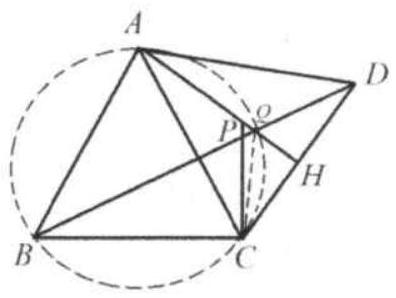
\includegraphics[width=\textwidth]{images/198.jpg}

Therefore, \(\angle A Q B=\angle A C B=60^{\circ}\).\\
\(\angle D Q=60^{\circ}\).\\
Since \(\angle Q H D=90^{\circ}, \angle B D C=90^{\circ}-60^{\circ}=30^{\circ}\).\\
Since \(\angle A C P=90^{\circ}-60^{\circ}=30^{\circ}, \angle A C P=\angle B D C\)

Since \(\angle A P C=90^{\circ}+\angle P C H, \angle B C D=90^{\circ}+\angle P C H, \angle A P C=\angle B C D\)\\
From (1) and (2): \(\triangle A P C \sim \triangle B C D\).\\
So \(\frac{A C}{B D}=\frac{A P}{B C} \Rightarrow A P \times B D=B C \times A C \Rightarrow\)\\
\(S_{A B C}=\frac{\sqrt{3}}{4} A C^{2}=\frac{\sqrt{3}}{4} B C \times A C=\frac{\sqrt{3}}{4} A P \times B D\).

Method 3:\\
We want to get: \(S=\frac{\sqrt{3}}{4} A P \times B D\).


We know that the area of any equilateral triangle with side length of \(a\) is:\\
\(S=\frac{\sqrt{3}}{4} a^{2}\), in our case, \(S=\frac{\sqrt{3}}{4} A B^{2}\).\\
We must have \(A B^{2}=A P \times B D \quad \Rightarrow \quad \frac{A B}{B D}=\frac{A P}{A B}\) or \(\frac{A C}{A P}=\frac{B D}{B C}\).\\
This is the ratio of two sides of two similar triangles \(\triangle A P C\) and \(\triangle B C D\) as shown. So we only need to prove that \(\triangle A P C \sim \triangle B C D\).\\
\centering
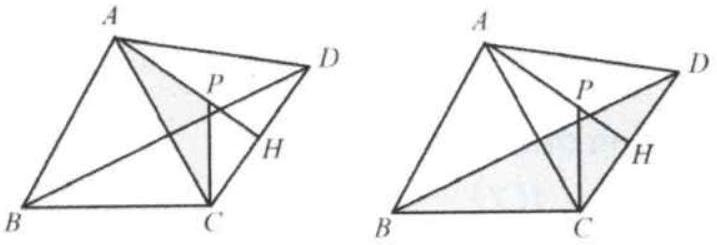
\includegraphics[width=\textwidth]{images/199(1).jpg}

We label each angle as shown below. We name the point of intersection of \(A C\) and \(B D\) be \(N\).\\
From triangle \(B A D\), We have\\
\(60^{\circ}+\alpha+\alpha+\gamma+\gamma=180^{\circ}\)\\
From triangles \(B N C, A N D\), We have\\
\(60^{\circ}+\theta=2 \alpha+\gamma\)\\
\centering
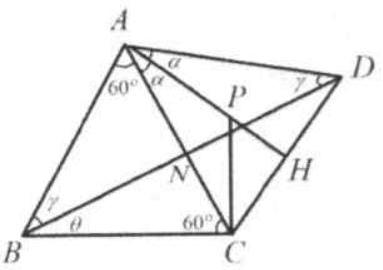
\includegraphics[width=\textwidth]{images/199.jpg}\\
(1) can be written as\\
\(\alpha+\gamma=60^{\circ}\)\\
From (2) and (3): \(\theta=\alpha\)\\
So we get \(\angle C A P=\angle C B D\). We need one more pair of congruent angles.\\
In right triangle \(A H D, \alpha+\gamma+\angle B D C=90^{\circ}(5)\)\\
Substituting (3) into (5): \(\angle B D C=30^{\circ}\).\\
Since \(C P \perp B C\) at \(C\) and \(\angle A C B=60^{\circ} . \angle A P C=30^{\circ}\).

Thus \(\triangle A P C \sim \triangle B C D\) and we are done.\\
Note: the first two solutions are official solution and the third one is our solution.


We know that \(\angle E A C=\angle E H C=\angle B D C=30^{\circ}\).\\
\(\angle P C A=90^{\circ}-60^{\circ}=30^{\circ}\). So \(\angle P C A=\angle B D C\).\\
Thus \(\triangle A C P \sim \triangle B D C\).\\
So \(\frac{A P}{B C}=\frac{A C}{B D} \Rightarrow A P \times B D=B C \times A C \Rightarrow\)\\
\(S_{A B C}=\frac{\sqrt{3}}{4} A C^{2}=\frac{\sqrt{3}}{4} B C \times A C=\frac{\sqrt{3}}{4} A P \times B D\).

Method 2:\\
Let the point of intersection of \(B D\) and \(A H\) be \(Q\).\\
Since \(A H \perp C D, A C=A D, \angle A C Q=\angle A D Q\).\\
Since \(A B=A D, \angle A D Q=\angle A B Q\).\\
\(\angle A B Q=\angle A C Q\).\\
Points \(A, B, C\), and \(Q\) are concyclic.\\
Therefore, \(\angle A Q B=\angle A C B=60^{\circ}\).\\
\centering
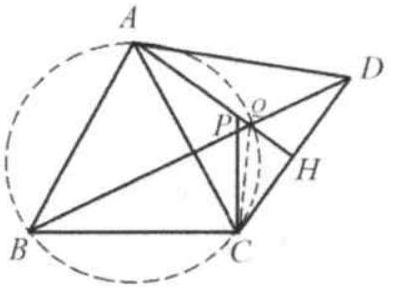
\includegraphics[width=\textwidth]{images/200.jpg}\\
\(\angle D Q=60^{\circ}\).\\
Since \(\angle Q H D=90^{\circ}, \angle B D C=90^{\circ}-60^{\circ}=30^{\circ}\).\\
Since \(\angle A C P=90^{\circ}-60^{\circ}=30^{\circ}, \angle A C P=\angle B D C\)

Since \(\angle A P C=90^{\circ}+\angle P C H, \angle B C D=90^{\circ}+\angle P C H, \angle A P C=\angle B C D\)\\
From (1) and (2): \(\triangle A P C \sim \triangle B C D\).\\
So \(\frac{A C}{B D}=\frac{A P}{B C} \Rightarrow A P \times B D=B C \times A C \Rightarrow\)\\
\(S_{A B C}=\frac{\sqrt{3}}{4} A C^{2}=\frac{\sqrt{3}}{4} B C \times A C=\frac{\sqrt{3}}{4} A P \times B D\).

Method 3:\\
We want to get: \(S=\frac{\sqrt{3}}{4} A P \times B D\).


We know that the area of any equilateral triangle with side length of \(a\) is: \(S=\frac{\sqrt{3}}{4} a^{2}\), in our case, \(S=\frac{\sqrt{3}}{4} A B^{2}\).\\
We must have \(A B^{2}=A P \times B D \quad \Rightarrow \quad \frac{A B}{B D}=\frac{A P}{A B}\) or \(\frac{A C}{A P}=\frac{B D}{B C}\).\\
This is the ratio of two sides of two similar triangles \(\triangle A P C\) and \(\triangle B C D\) as shown. So we only need to prove that \(\triangle A P C \sim \triangle B C D\).\\
\centering

\includegraphics[width=\textwidth]{images/201.jpg}

We label each angle as shown below. We name the point of intersection of \(A C\) and \(B D\) be \(N\).\\
From triangle \(B A D\), We have\\
\(60^{\circ}+\alpha+\alpha+\gamma+\gamma=180^{\circ}\)\\
From triangles \(B N C, A N D\), We have\\
\(60^{\circ}+\theta=2 \alpha+\gamma\)\\
(1) can be written as\\
\centering
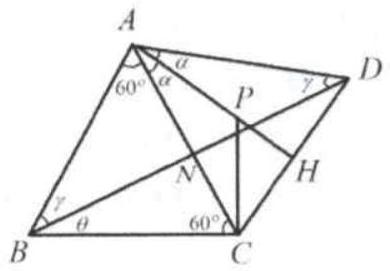
\includegraphics[width=\textwidth]{images/201(1).jpg}\\
\(\alpha+\gamma=60^{\circ}\)\\
From (2) and (3): \(\theta=\alpha\)

So we get \(\angle C A P=\angle C B D\). We need one more pair of congruent angles.\\
In right triangle \(A H D, \alpha+\gamma+\angle B D C=90^{\circ}(5)\)

Substituting (3) into (5): \(\angle B D C=30^{\circ}\).

Since \(C P \perp B C\) at \(C\) and \(\angle A C B=60^{\circ} . \angle A P C=30^{\circ}\).

Thus \(\triangle A P C \sim \triangle B C D\) and we are done.\\
Note: the first two solutions are official solution and the third one is our solution.



\end{document}
